%! TEX root = ../main.tex
\chapter{The {\gerda} experiment}
The {\gerda} experiment (GERmanium Detector Array) is a search for the neutrinoless double-beta ($0\nbb$) decay of \ce{^{76}Ge}. As we saw in the previous chapter, the half lives for $0\nbb$ decay, assuming the process exists, are expected to be substantially longer than the corresponding $2\nbb$ ones. Consequently, $0\nbb$ decay experiments must be sensitive to just a few events per year for a source with a mass of tens to hundreds of kilograms. Backgrounds must typically be reduced to the level of one event per year in the region of interest, an energy interval of the order of the energy resolution around $Q_{\beta\beta}$. 

Experiments looking for $0\nbb$ decay of \ce{^{76}Ge} operate germanium diodes normally made from enriched material, i.e.~the number of \ce{^{76}Ge} nuclei, the isotopic fraction $f_{76}$, is enlarged from 7.8\% to 86\% or higher. In these type of experiments, the source is equal to the detector which yields high detection efficiency. Additional advantages of this technique are the superior energy resolution of 0.2\% at $Q_{\beta\beta}=2039$ keV compared to other searches with different isotopes and the high radiopurity of the crystal growing procedure. Disadvantages are the relatively low $Q_{\beta\beta}$ value since backgrounds typically fall with energy and the relative difficulty to scale to larger mass compared to e.g.~experiments using liquids and gases.

{\gerda} has been built in the INFN Laboratori Nazionali del Gran Sasso (LNGS) at a depth of 3500 m w.e.~(water equivalent) and submerses bare high-purity germanium detectors enriched in \ce{^{76}Ge} into liquid argon (LAr). LAr serves simultaneously as a shield against external radioactivity and as cooling medium. Phase \textsc{i} of the experiment was planned to give a statistically unambiguous statement concerning the observation of of the neutrinoless double-beta decay claimed by a subgroup of the \textsc{HdM} collaboration \cite{hdmclaim} and establish the quality cuts on the data. It ended in may 2013 with a total exposure of 21.6 kg$\cdot$yr, the analysis reported no excess of events above the background at $Q_{\beta\beta}$ \cite{Agostini:2013mzu}, with a corresponding half-life of
\[T_{1/2}^{0\nbb}>2.1\cdot10^{25}\;\text{yr}\qquad\text{(90\% C.L.)}\;.\]
Phase \textsc{ii} of {\gerda} is planned to acquire an exposure of 100 kg$\cdot$yr to improve the sensitivity and study the properties of the neutrino mass.

\marginnote{\textsc{Design and General Layout}} The main feature of the {\gerda} design is to operate bare Ge detectors made out of material enriched in \ce{^{76}Ge} (\ce{^{enr}Ge}) in LAr. It allows for a significant reduction in the cladding material around the diodes and the accompanying radiation sources as compared to traditional Ge experiments. Furthermore, the background produced by interactions of cosmic rays is lower than for the traditional concepts due to the lower $Z$ of the shielding material. Other background sources include neutrons and gammas from the decays in the rock of the underground laboratory, radioactivity in support materials, radioactive elements in the cryogenic liquid as well as internal backgrounds in the Ge diodes. Natural Ge (\ce{^{nat}Ge}) contains about 7.8\% \ce{^{76}Ge}, and could in principle be used directly for a $0\nbb$ decay experiment. However enriched detectors allow for a better signal-to-background ratio and also yield reduced costs for a fixed mass of \ce{^{76}Ge} in the experiment.
\begin{figure}
	\centering
	\begin{tikzpicture}[fill=white]
		\node at (0,0) {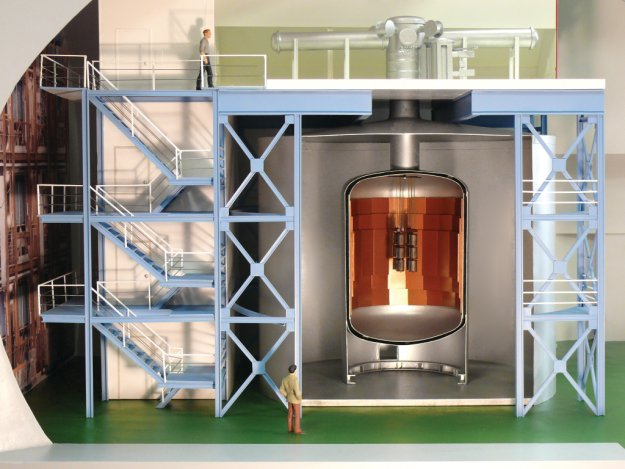
\includegraphics[width=\textwidth]{img/GERDAmodel}};
		\node(a) at (1.9,-1.5) [rectangle,draw,fill] {LAr};
		\node(b) at (4,1.6) [rectangle,draw,fill] {\ce{^76Ge} \textsc{detectors}};
		\draw[thick,red,->] (b.south) .. controls +(0,0) and +(1,0) .. (1.9,-0.4);
		\node(c) at (-1.5,1.6) [rectangle,draw,fill] {\textsc{water tank}};
		\draw[thick,red,->] (c.south) .. controls +(0,0) and +(-1,0) .. (0,-1);
		\node(d) at (0,3) [rectangle,draw,fill] {\textsc{copper shielding}};
		\draw[thick,red,->] (d.south) .. controls +(0,0) and +(-1,0) .. (1,0);
	\end{tikzpicture}
	\caption{Artists view (Ge array not to scale) of the Gerda experiment.}
	\label{artistview}
\end{figure}
\begin{figure}
	\centering
	\resizebox{\textwidth}{!}{
		\includegraphics[height=15cm]{img/strings}%
		\hspace{0.1cm}%
		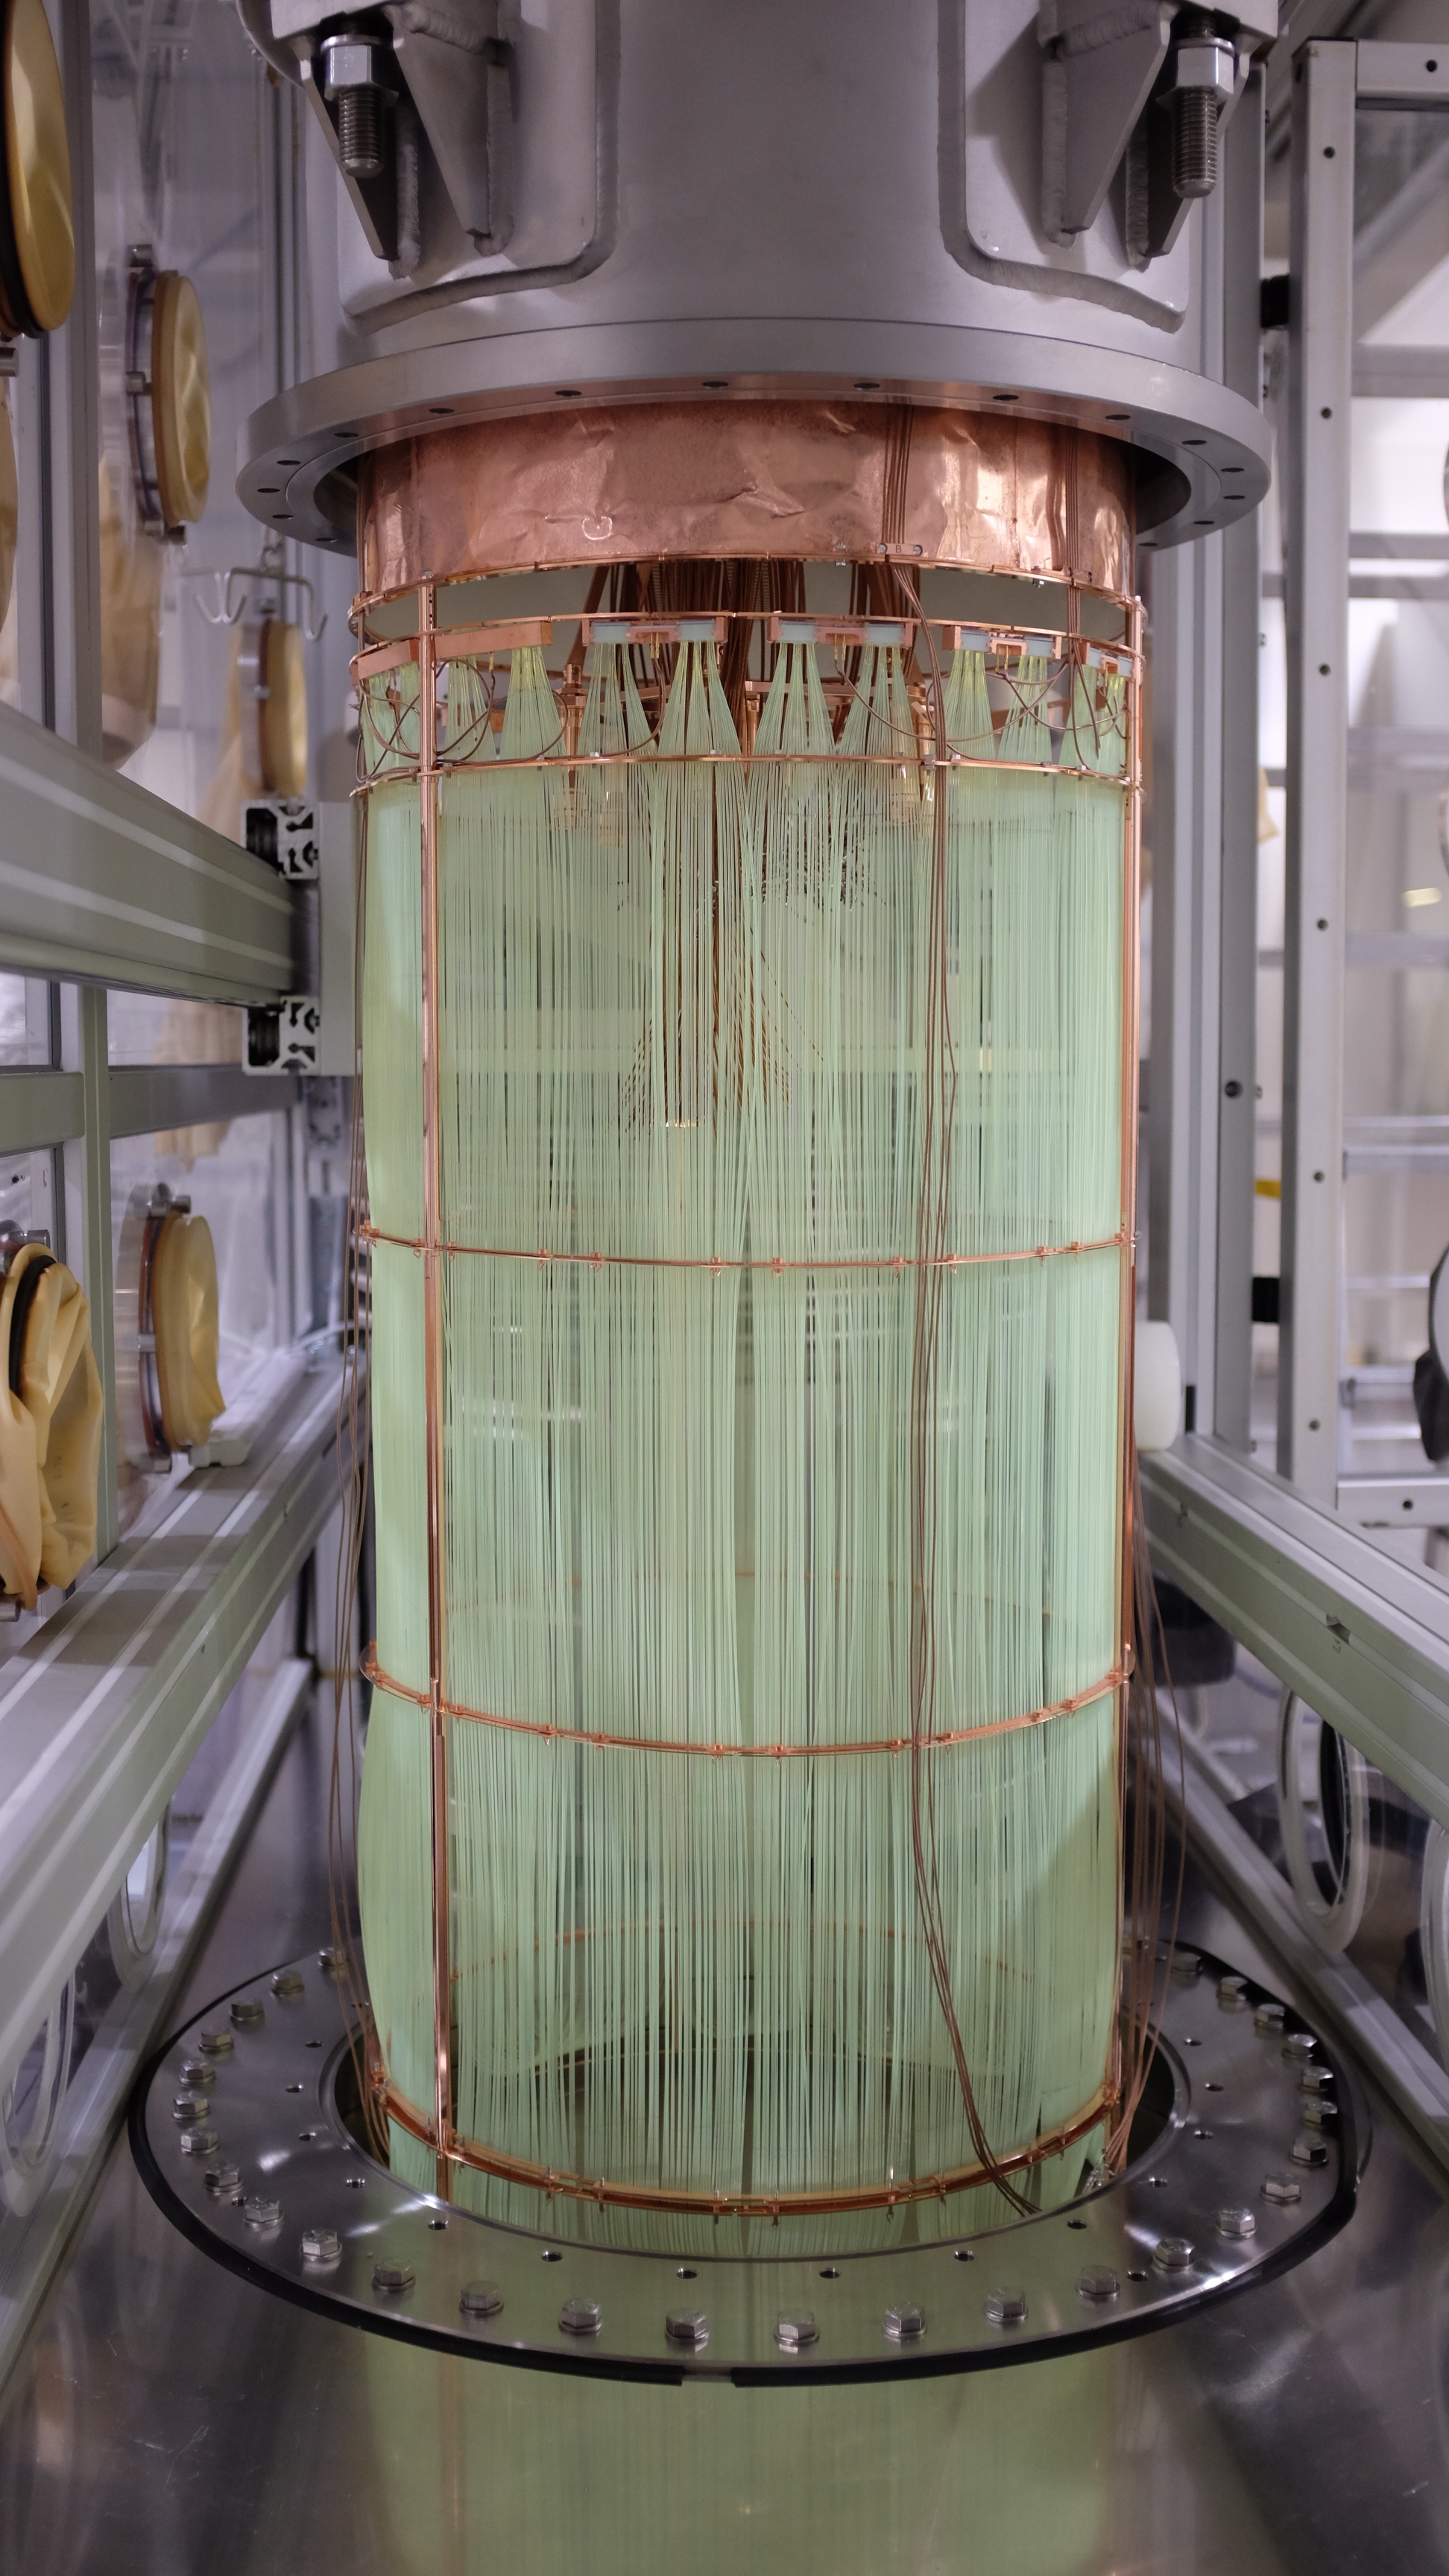
\includegraphics[height=15cm]{img/fibers}%
	}%
	\caption{On the left: some detector strings. On the right: the fiber shroud being submerged in LAr?}
\end{figure}
\begin{figure}
	\centering
	\makebox[\textwidth]{\includegraphics[width=\textwidth]{img/water_tank}}
	\caption{Inside the water tank after the installation of the muon veto system.}
\end{figure}

Fig.~\ref{artistview} shows a model of the realized design: the core of the experiment is an array of germanium diodes suspended in strings into a cryostat filled with LAr. The LAr serves both as cooling medium and shield. The cryostat is a steel vessel with a copper lining used primarily to reduce the gamma radiation from the steel vessel. The cryostat is placed in a large water tank, that fulfills the functions of shielding the inner volumes from radiation sources within the hall, such as neutrons, as well as providing a sensitive medium for a muon veto system. The detectors are lowered into the LAr volume using a lock system located in a clean room on top of the water tank. A further muon veto system is placed on top of the clean room in order to shield the neck region of the cryostat. A detailed description of the experimental setup for phase \textsc{i} is provided in \cite{gerdadescription}.

Phase \textsc{ii} came with some upgrades to improve the background rejection performance. The volume directly surrounding the detector array was instrumented with photo multipliers to detect the scintillation light emitted if energy is deposited inside LAr. This allows to identify background events resulting from Compton scattered photons with partial energy deposit in the detectors and partial energy deposit inside the LAr. Additionally, a curtain made from light guide fibers with tetraphenyl butadiene (TPB) deposited on their surface will surround the detector array. Photons reaching the light guides are wavelength shifted and guided to the end of the fibers, where they can be detected by silicon photomultipliers (SiPMs) optically coupled to the fibers. In principle the new components should improve the identification of background events. In Phase \textsc{i} the individual detector strings were surrounded by a copper shroud, minimizing the LAr volume from which \ce{^{42}K} ions can be collected on the detector surfaces. Additionally the shrouds were set to ground potential to minimize drift towards the detectors. In order to take maximum advantage of the light instrumentation of the LAr, in Phase \textsc{ii} the copper shroud has been be exchanged by a transparent TPB-coated shroud that allows to minimize the volume from which \ce{^{42}K} ions are collected, while allowing to detected scintillation light also from the volume inside the mini shroud. Last but not least, 30 new BEGe detectors were deployed into the LAr.

\marginnote{\textsc{The germanium detectors}} For Phase \textsc{i} all eight detectors from the former \textsc{HdM} \cite{hdm}and \textsc{Igex} \cite{igex} experiments were refurbished and redeployed, In addition, six detectors made of \ce{^{na}Ge} are available from the GENIUS-TF experiment \cite{genius1, genius2}. For Phase \textsc{ii} new material amounting to 50 kg \ce{^{enr}GeO2} was purchased in order to produce new diodes.
